% !TeX root = ../../Skript.tex
\cohead{\Large\textbf{Verhalten für \(x\to \pm \infty \)}}
\fakesubsection{Verhalten für \texorpdfstring{\(x\to \pm \infty \)}{sehr große/kleine x}}
\begin{tcolorbox}\centering
	\textcolor{loestc}{Eine ganzrationale Funktion \(f(x)\) verhält sich für sehr große bzw. sehr kleine \(x\) wie\\ \(\text{Leitkoeffizient}\cdot x^{\text{Grad}}\)}

\end{tcolorbox}
\begin{minipage}{\textwidth}
	\adjustbox{valign=t}{\begin{minipage}{0.33\textwidth}\centering
		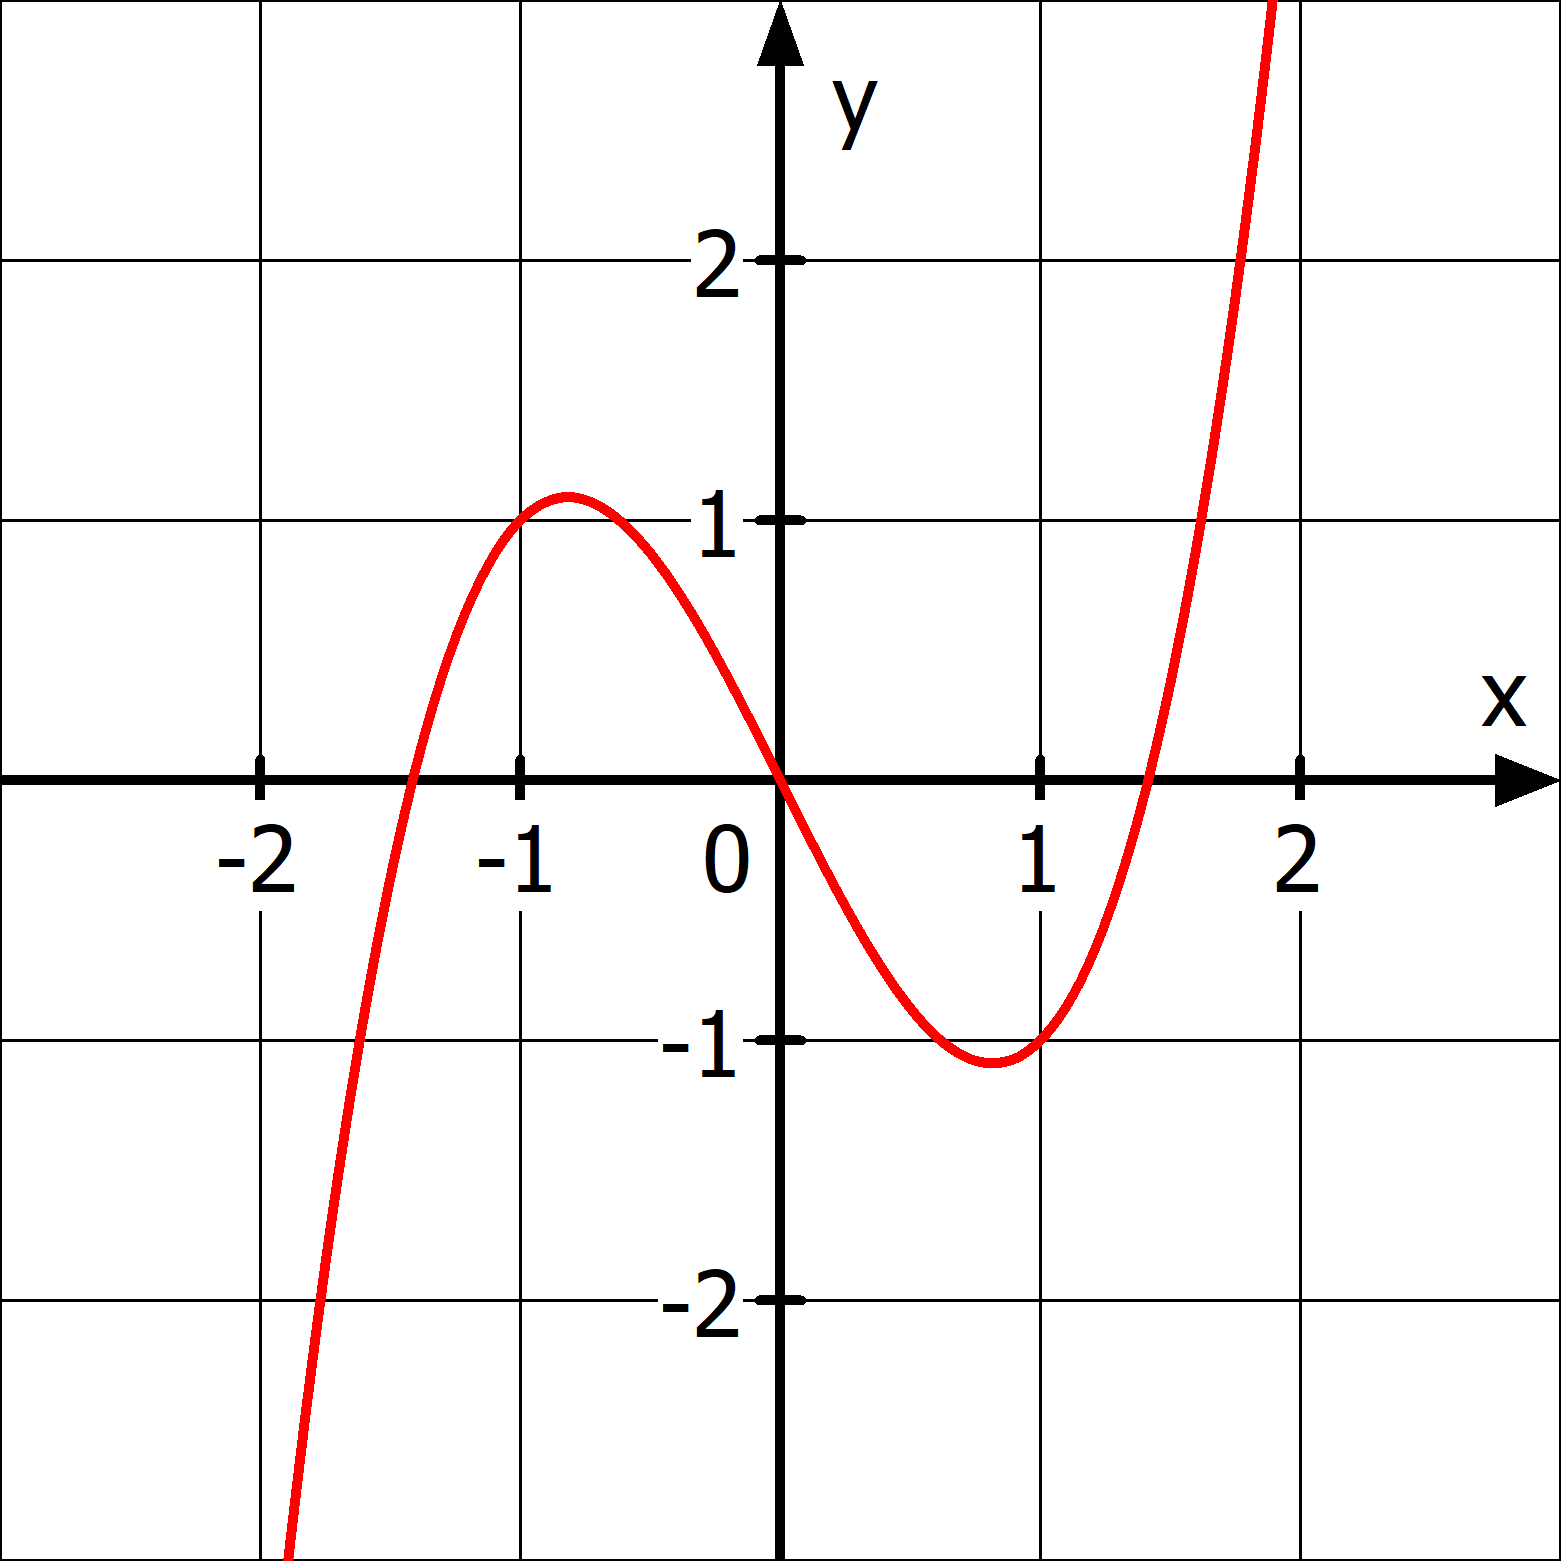
\includegraphics[width=.87\textwidth]{\ganzFkt/pics/sym4.png}

		\(f_1(x)=x^3-2x\)

		\textcolor{loes}{\(f_1(x)\xrightarrow{\hphantom{\ }x\to-\infty\hphantom{\ }}-\infty\)}

		\textcolor{loes}{\(f_1(x)\xrightarrow{\hphantom{\ }x\to\infty\hphantom{\ }}\infty\)}

		\textcolor{loes}{Verhält sich wie \(x^3\)}
	\end{minipage}}%
	\adjustbox{valign=t}{\begin{minipage}{0.33\textwidth}\centering
		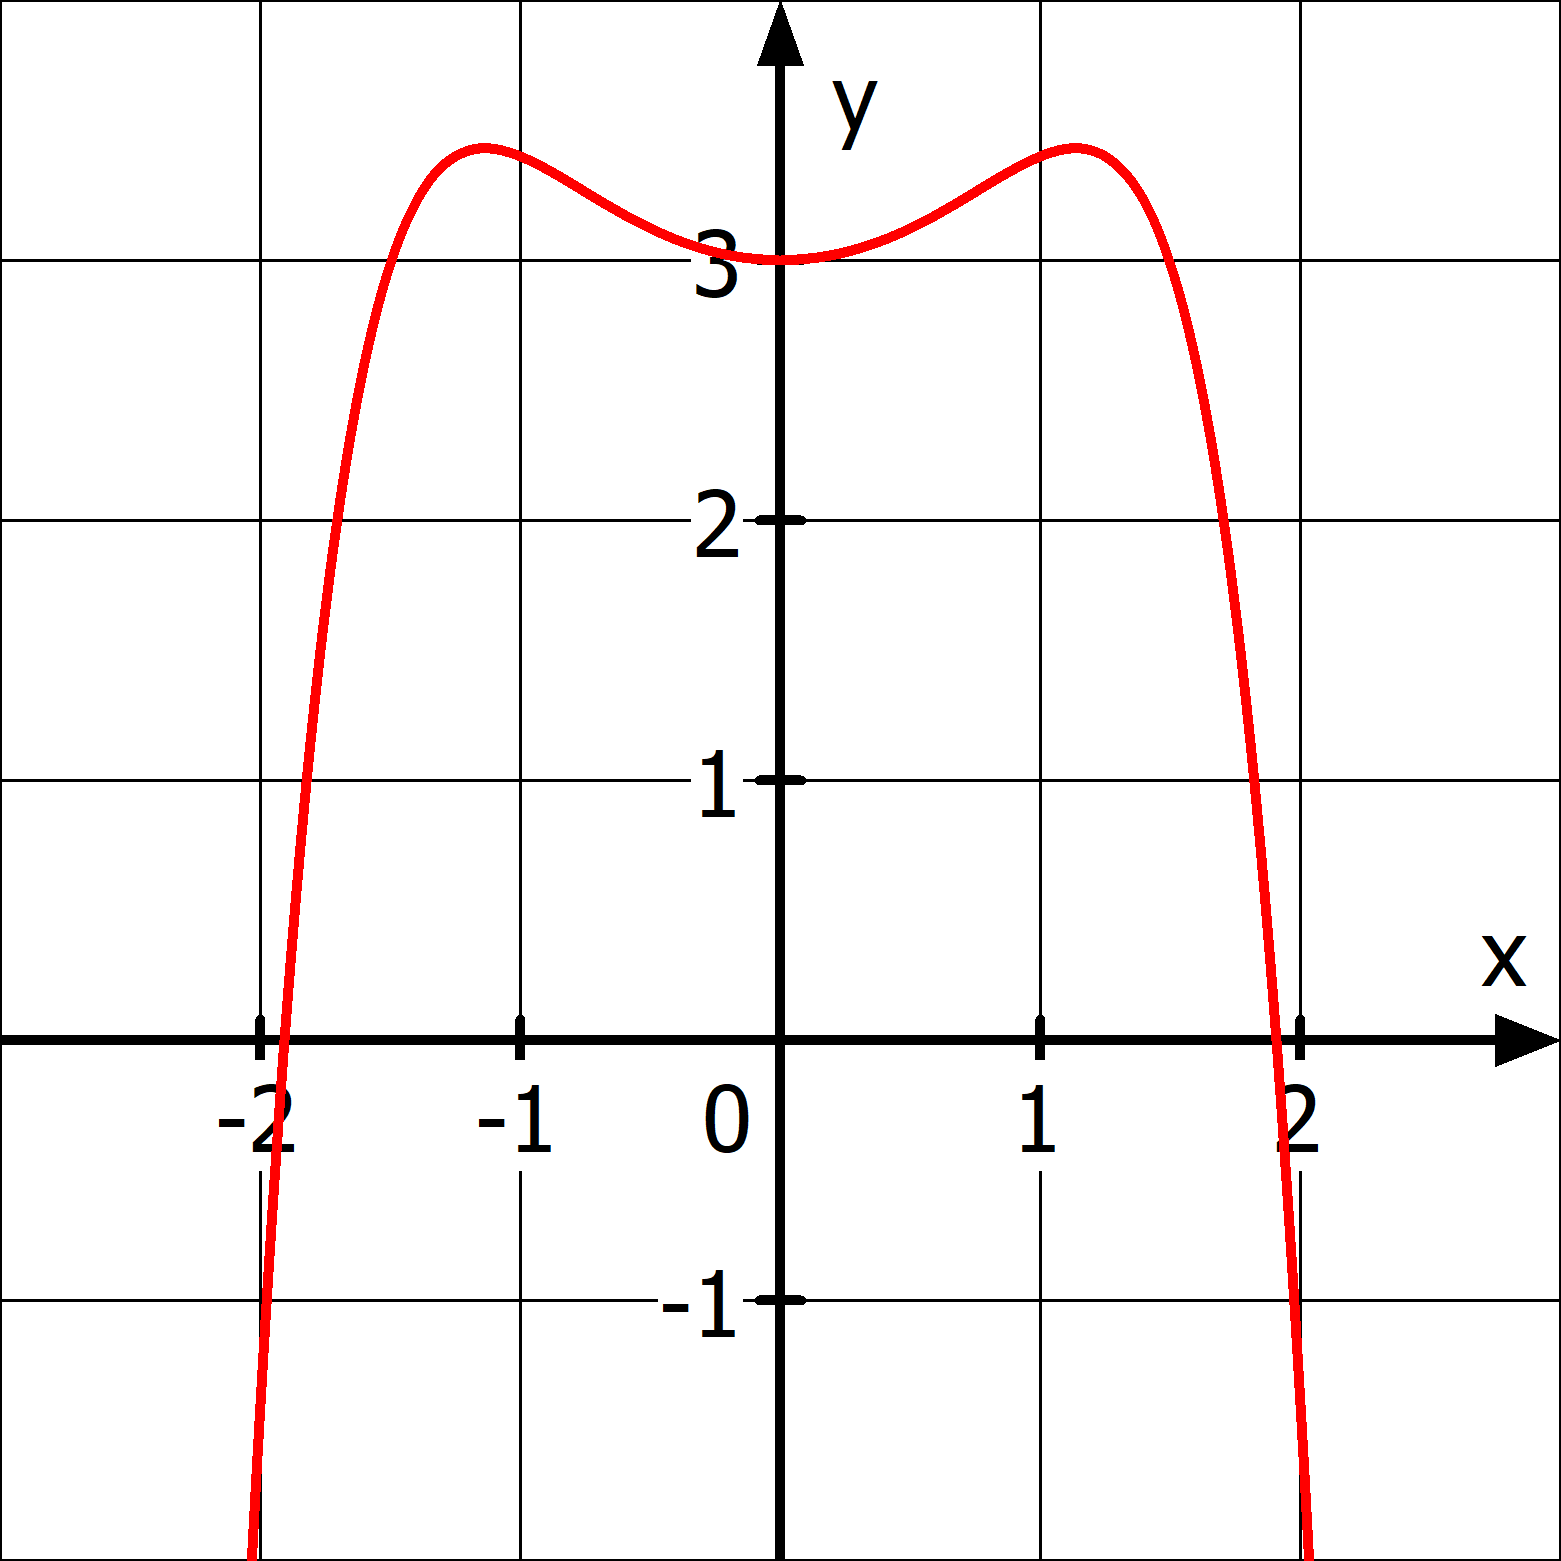
\includegraphics[width=.87\textwidth]{\ganzFkt/pics/sym2.png}

		\(f_2(x)=-0,1x^6+0,5x^2+3\)

		\textcolor{loes}{\(f_2(x)\xrightarrow{\hphantom{\ }x\to-\infty\hphantom{\ }}-\infty\)}

		\textcolor{loes}{\(f_2(x)\xrightarrow{\hphantom{\ }x\to\infty\hphantom{\ }}-\infty\)}

		\textcolor{loes}{Verhält sich wie \(-0,1x^6\)}
	\end{minipage}}%
	\adjustbox{valign=t}{\begin{minipage}{0.33\textwidth}\centering
		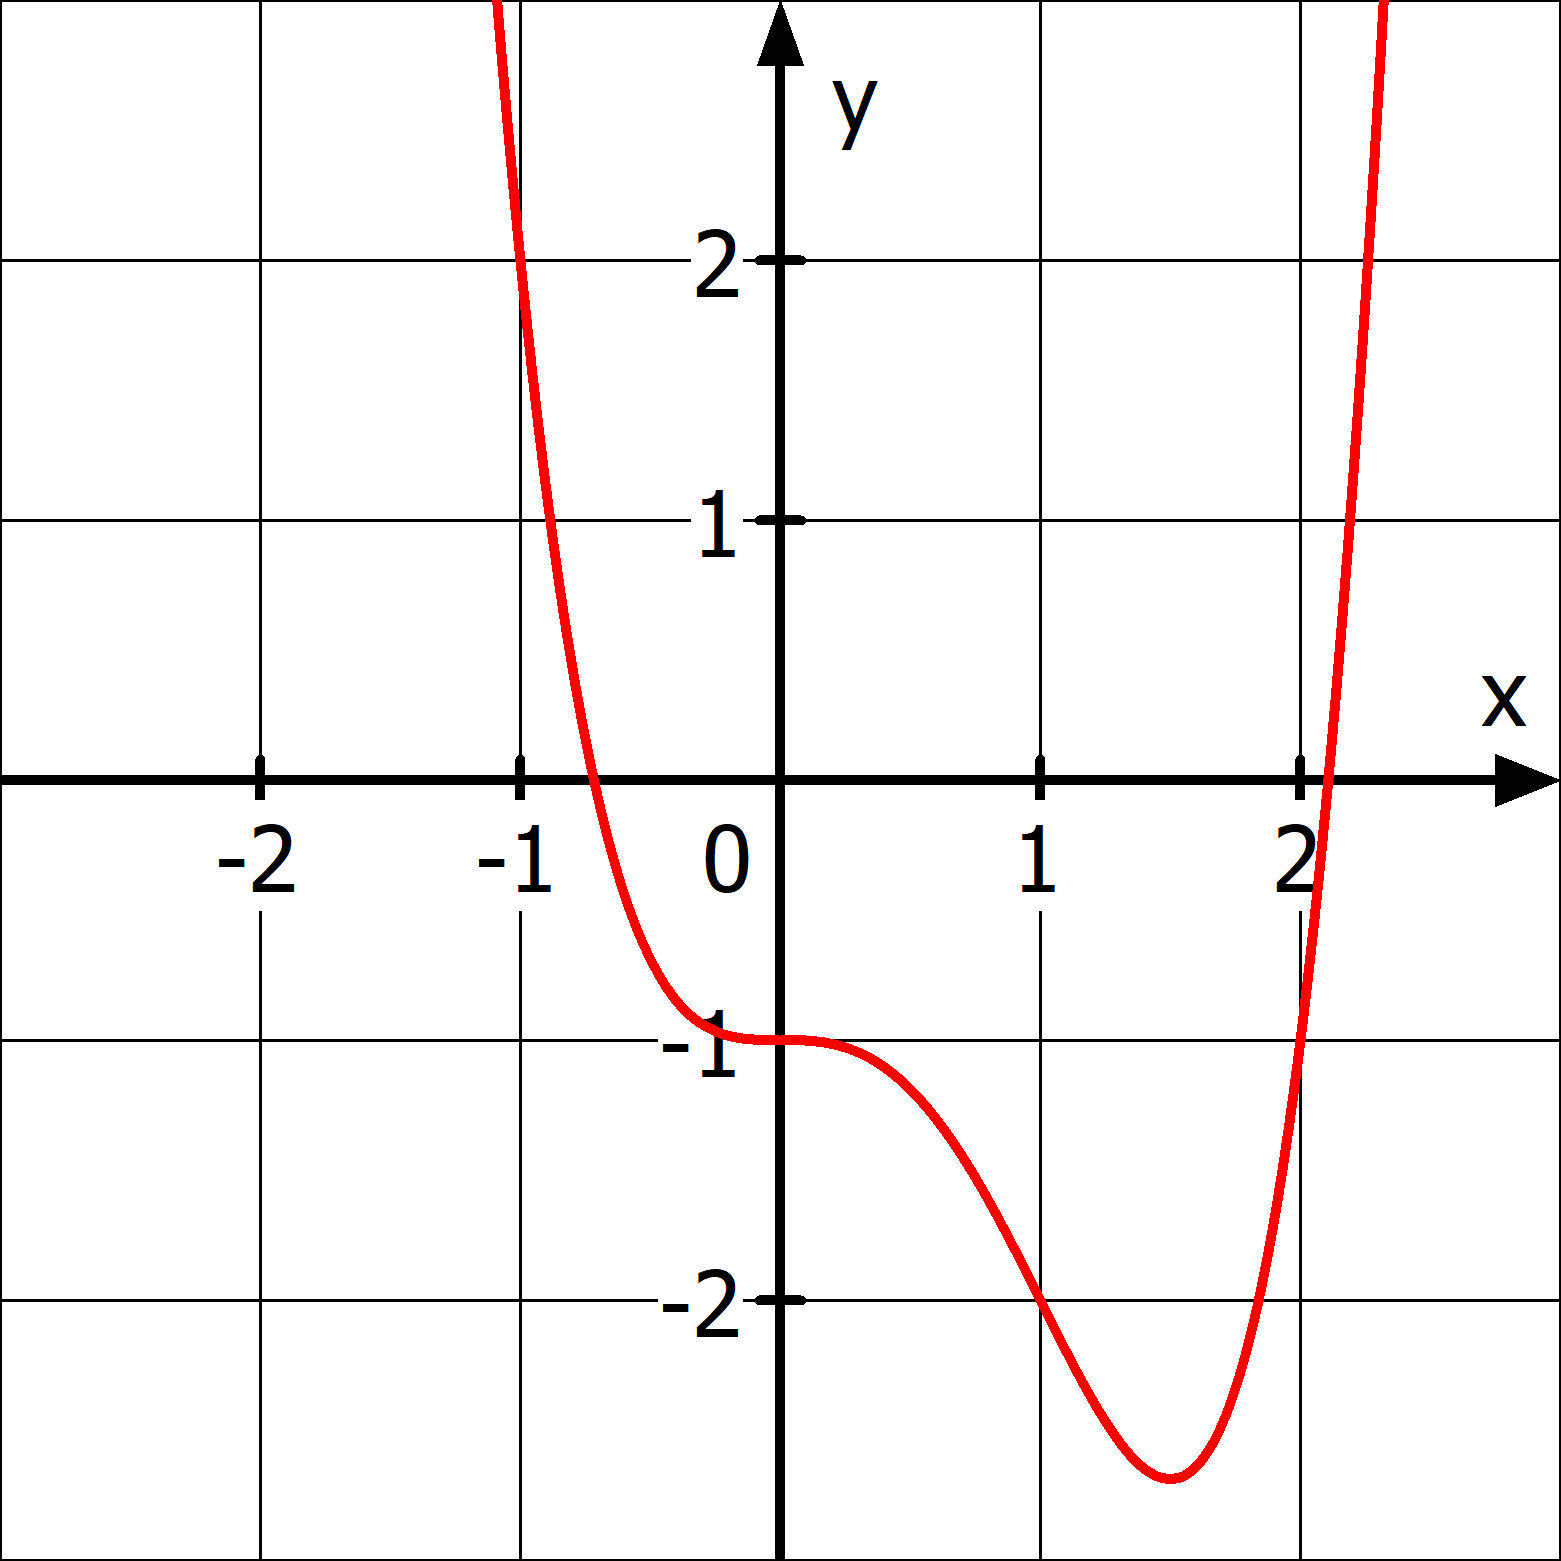
\includegraphics[width=.87\textwidth]{\ganzFkt/pics/sym8.png}

		\(f_3(x)=x^4-2x^3-1\)

		\textcolor{loes}{\(f_3(x)\xrightarrow{\hphantom{\ }x\to-\infty\hphantom{\ }}\infty\)}

		\textcolor{loes}{\(f_3(x)\xrightarrow{\hphantom{\ }x\to\infty\hphantom{\ }}\infty\)}

		\textcolor{loes}{Verhält sich wie \(x^4\)}
	\end{minipage}}%
\end{minipage}

%%%%%%%%%%%%%%%%%%%%%%%%%%%%%%%%%%%%%%%%%%%%%%%%%%%%%%%%%%%%%%
\begin{minipage}{\textwidth}
	\adjustbox{valign=t}{\begin{minipage}{0.32\textwidth}\centering
		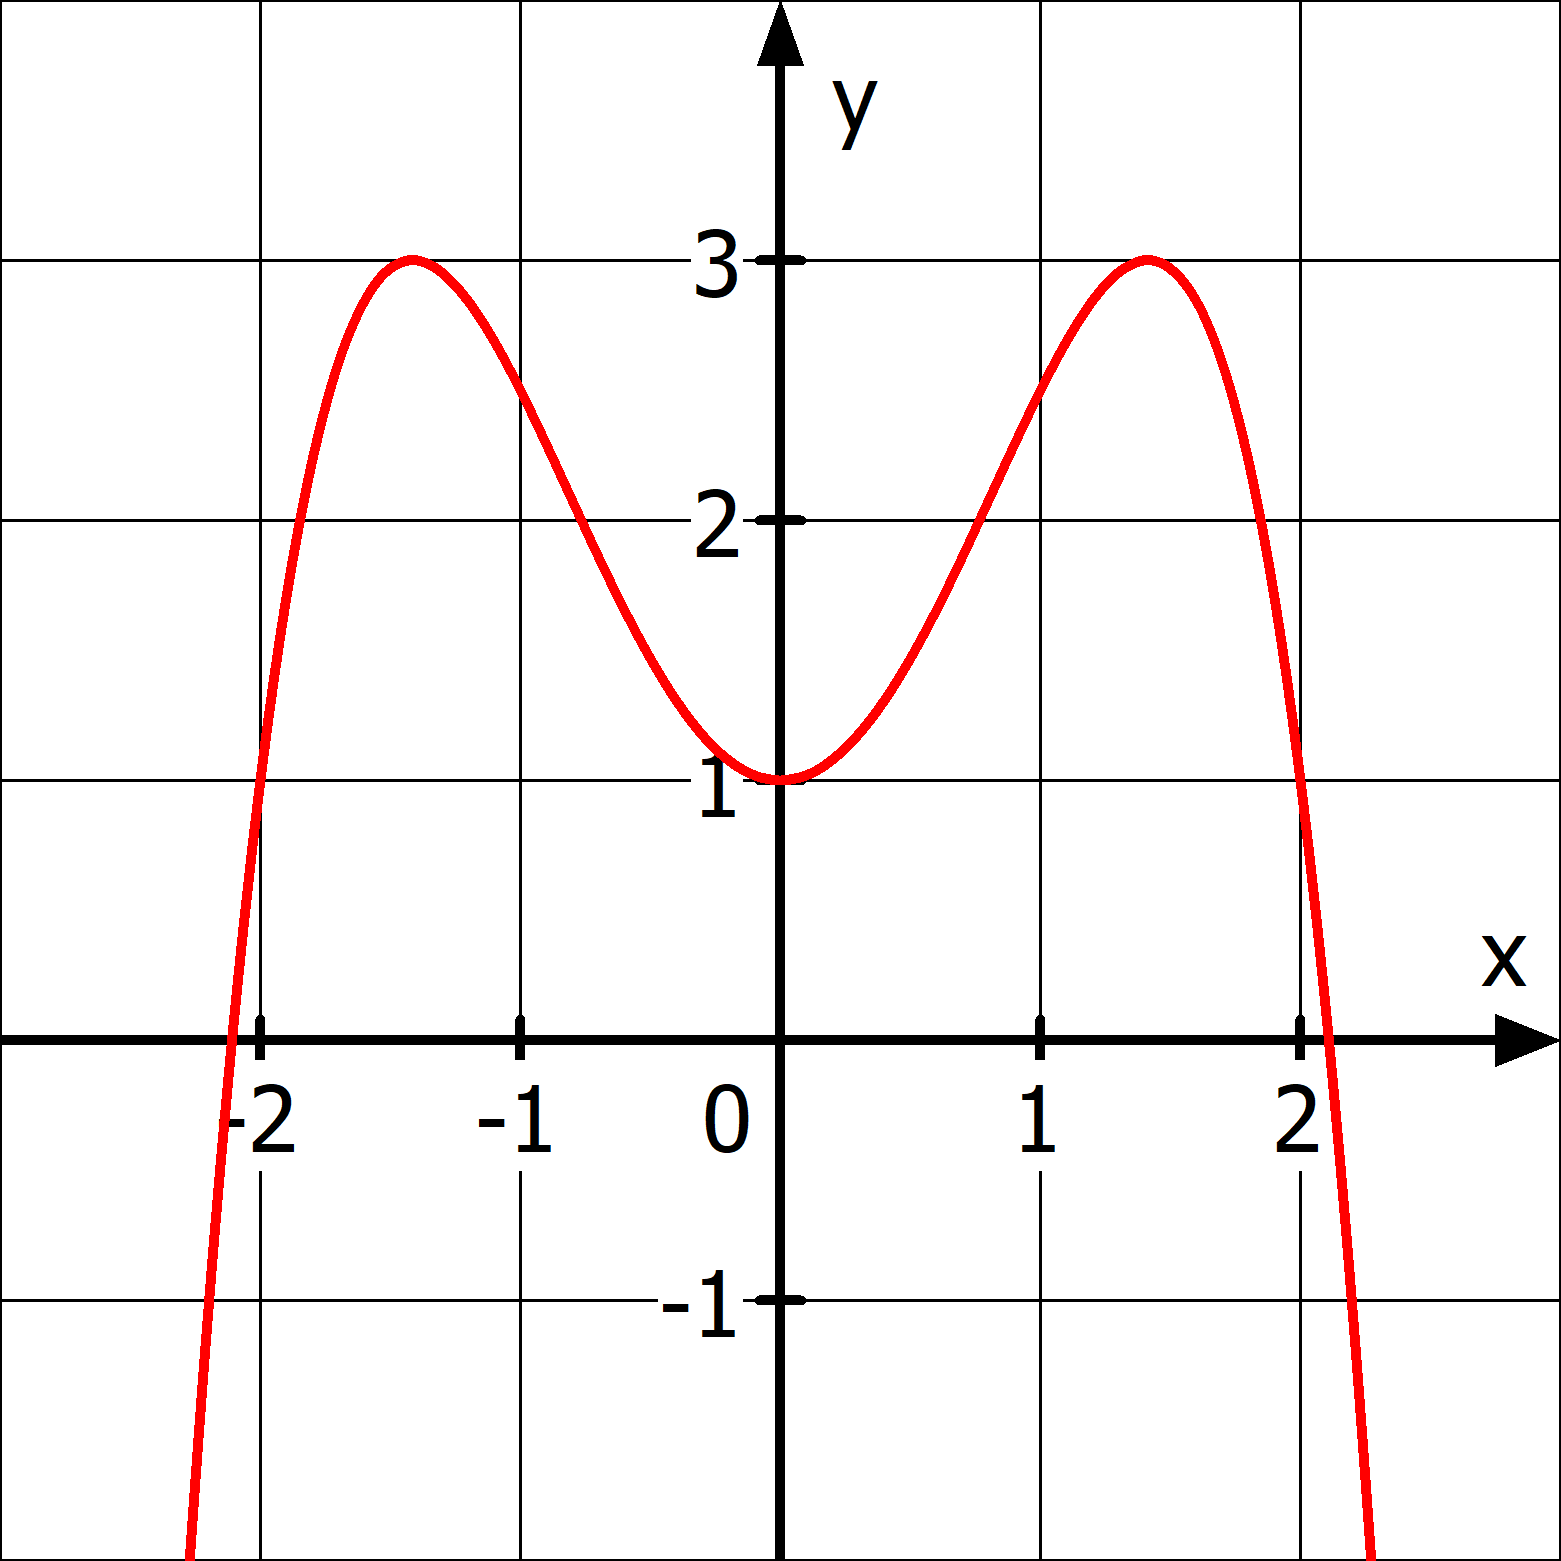
\includegraphics[width=.87\textwidth]{\ganzFkt/pics/sym1.png}

		\(f_4(x)= -\frac{1}{2}x^4+2x^2+1\)

		\textcolor{loes}{\(f_4(x)\xrightarrow{\hphantom{\ }x\to-\infty\hphantom{\ }}-\infty\)}

		\textcolor{loes}{\(f_4(x)\xrightarrow{\hphantom{\ }x\to\infty\hphantom{\ }}-\infty\)}

		\textcolor{loes}{Verhält sich wie \(-\frac{1}{2}x^4\)}
	\end{minipage}}%
	\adjustbox{valign=t}{\begin{minipage}{0.33\textwidth}\centering
		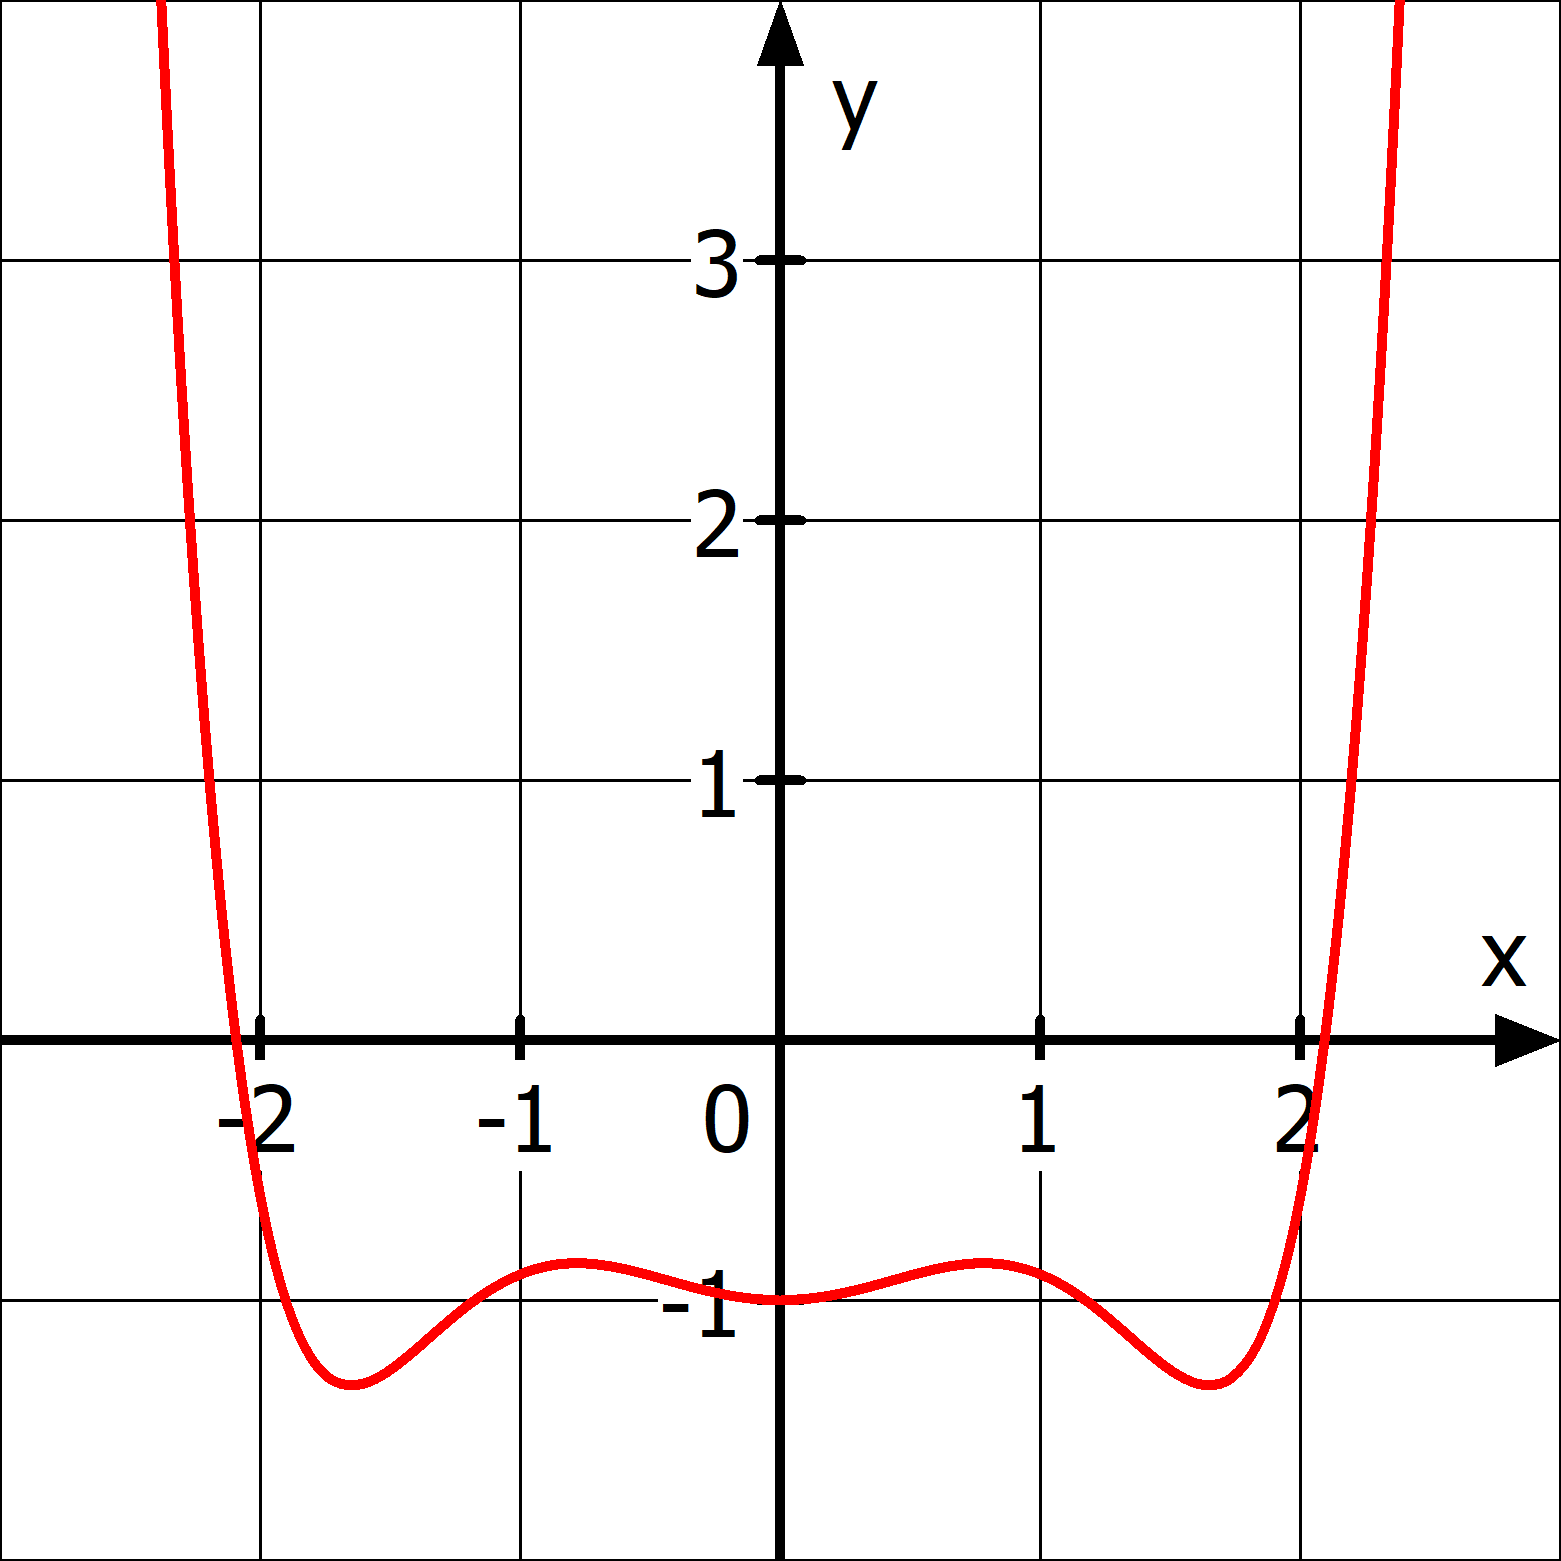
\includegraphics[width=.87\textwidth]{\ganzFkt/pics/sym3.png}

		\(f_5(x)=\frac{1}{10}x^6-\frac{1}{2}x^4+\frac{1}{2}x^2-1\)

		\textcolor{loes}{\(f_5(x)\xrightarrow{\hphantom{\ }x\to-\infty\hphantom{\ }}\infty\)}

		\textcolor{loes}{\(f_5(x)\xrightarrow{\hphantom{\ }x\to\infty\hphantom{\ }}\infty\)}

		\textcolor{loes}{Verhält sich wie \(\frac{1}{10}x^6\)}
	\end{minipage}}%
	\adjustbox{valign=t}{\begin{minipage}{0.33\textwidth}\centering
		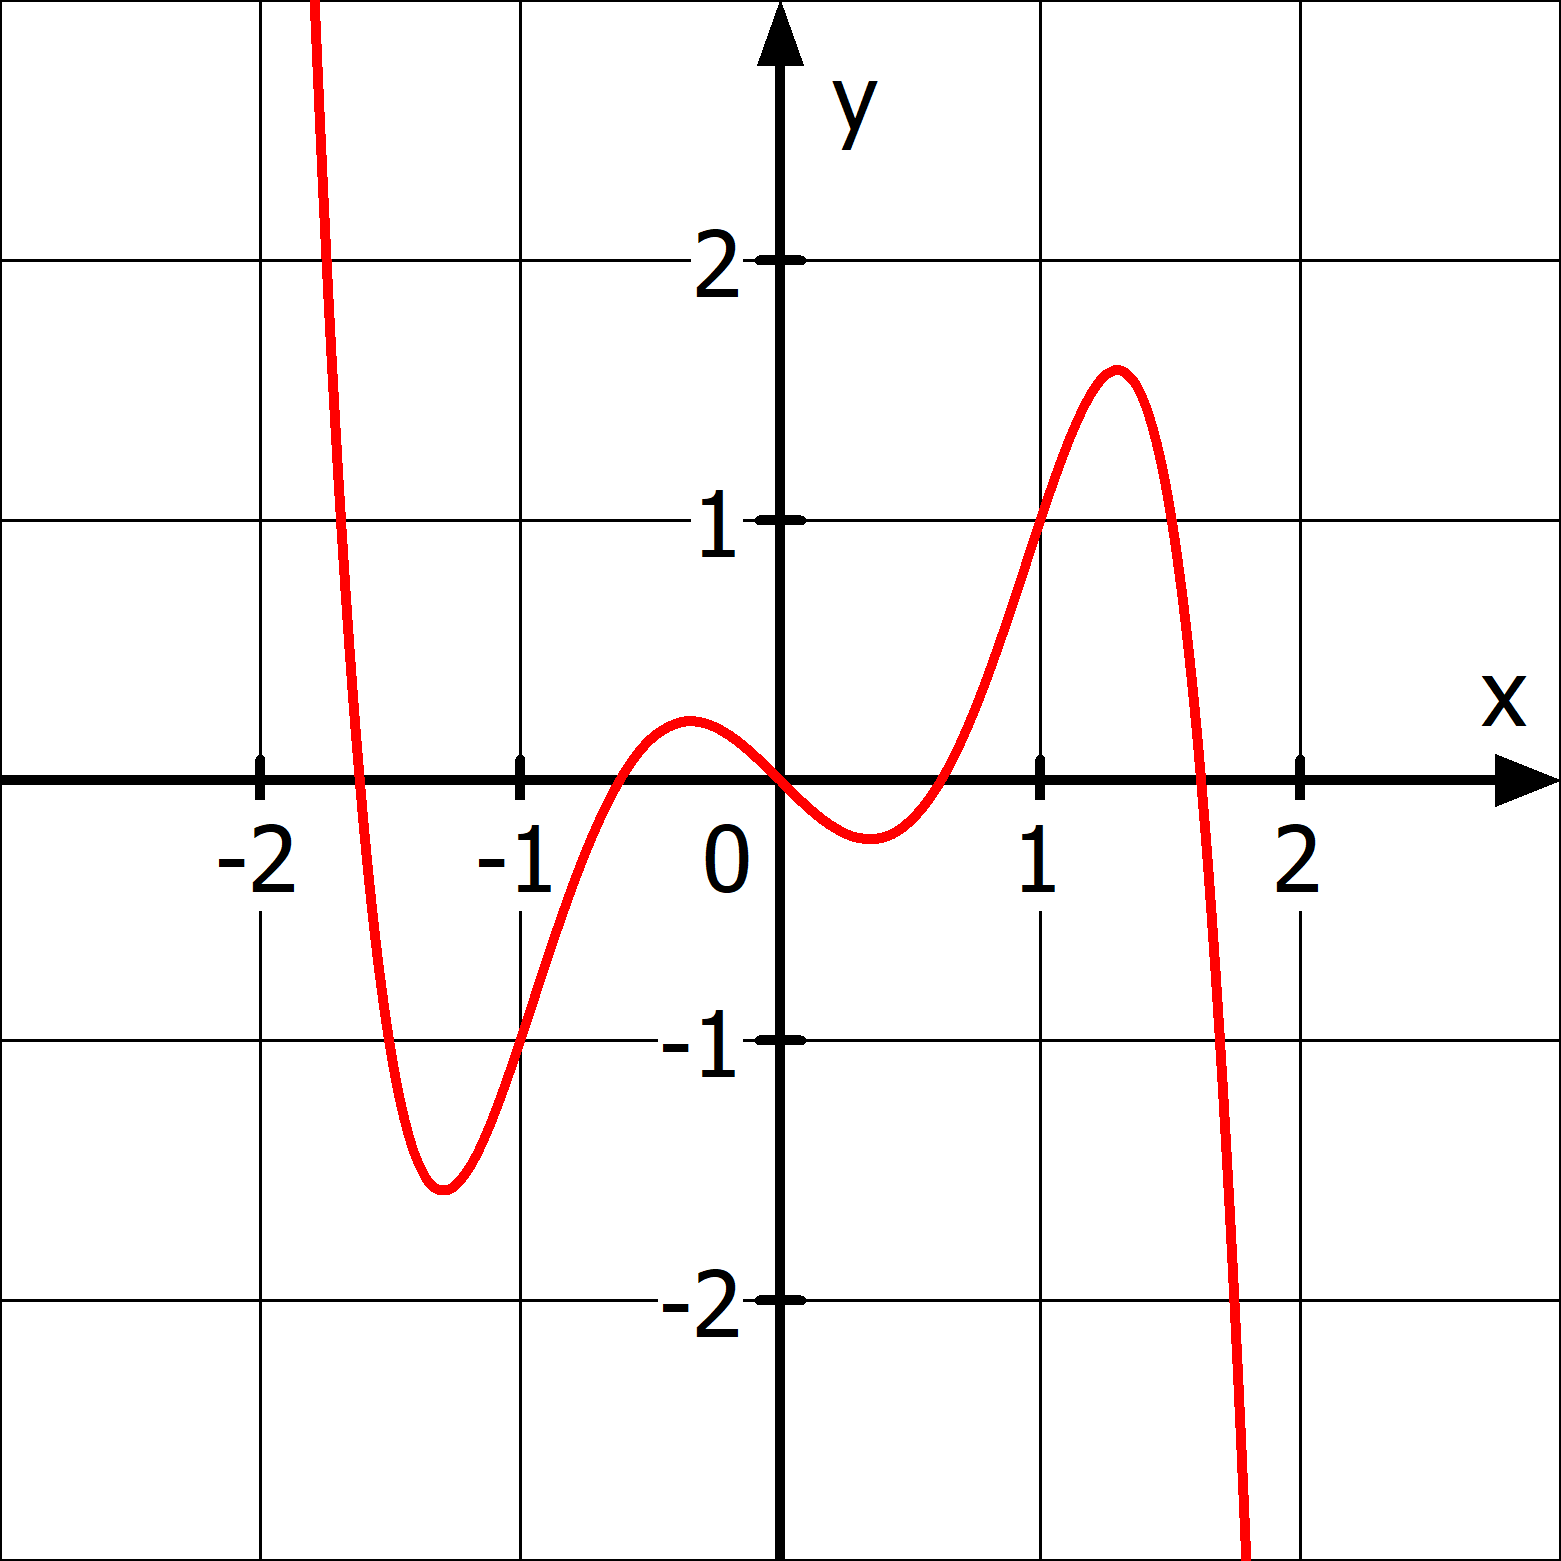
\includegraphics[width=.87\textwidth]{\ganzFkt/pics/sym5.png}

		\(f_6(x)=-x^5+3x^3-x\)

		\textcolor{loes}{\(f_6(x)\xrightarrow{\hphantom{\ }x\to-\infty\hphantom{\ }}\infty\)}

		\textcolor{loes}{\(f_6(x)\xrightarrow{\hphantom{\ }x\to\infty\hphantom{\ }}-\infty\)}

		\textcolor{loes}{Verhält sich wie \(-x^5\)}
	\end{minipage}}%
\end{minipage}

%%%%%%%%%%%%%%%%%%%%%%%%%%%%%%%%%%%%%%%%%%%%%%%%%%%%%%%%%%%%%%
\begin{minipage}{\textwidth}
	\adjustbox{valign=t}{\begin{minipage}{0.33\textwidth}\centering
		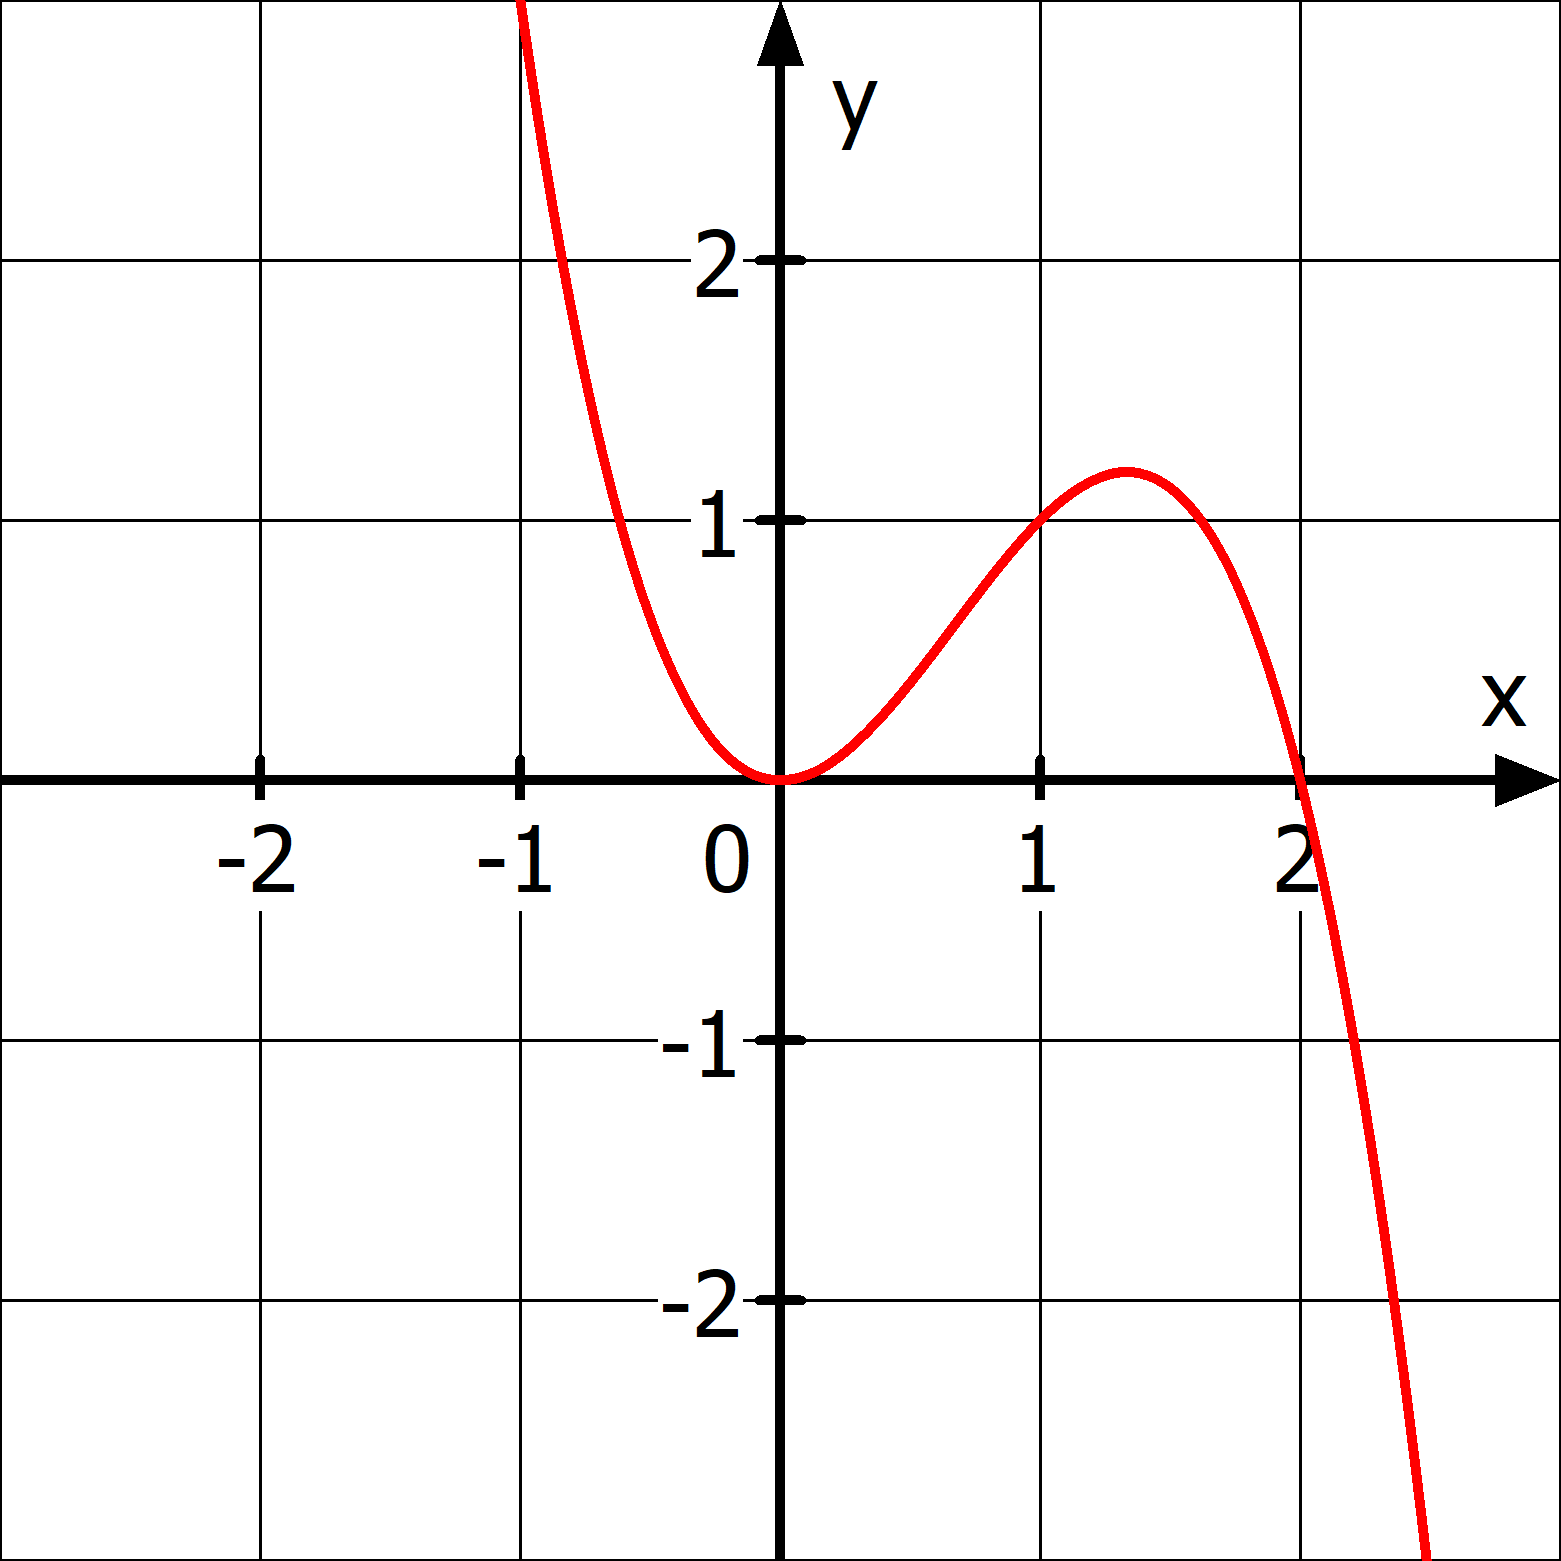
\includegraphics[width=.87\textwidth]{\ganzFkt/pics/sym7.png}

		\(f_7(x)=-x^3+2x^2\)\\
		\textcolor{loes}{\(f_7(x)\xrightarrow{\hphantom{\ }x\to-\infty\hphantom{\ }}\infty\)}

		\textcolor{loes}{\(f_7(x)\xrightarrow{\hphantom{\ }x\to\infty\hphantom{\ }}-\infty\)}

		\textcolor{loes}{Verhält sich wie \(-x^3\)}
	\end{minipage}}%
	\adjustbox{valign=t}{\begin{minipage}{0.33\textwidth}\centering
		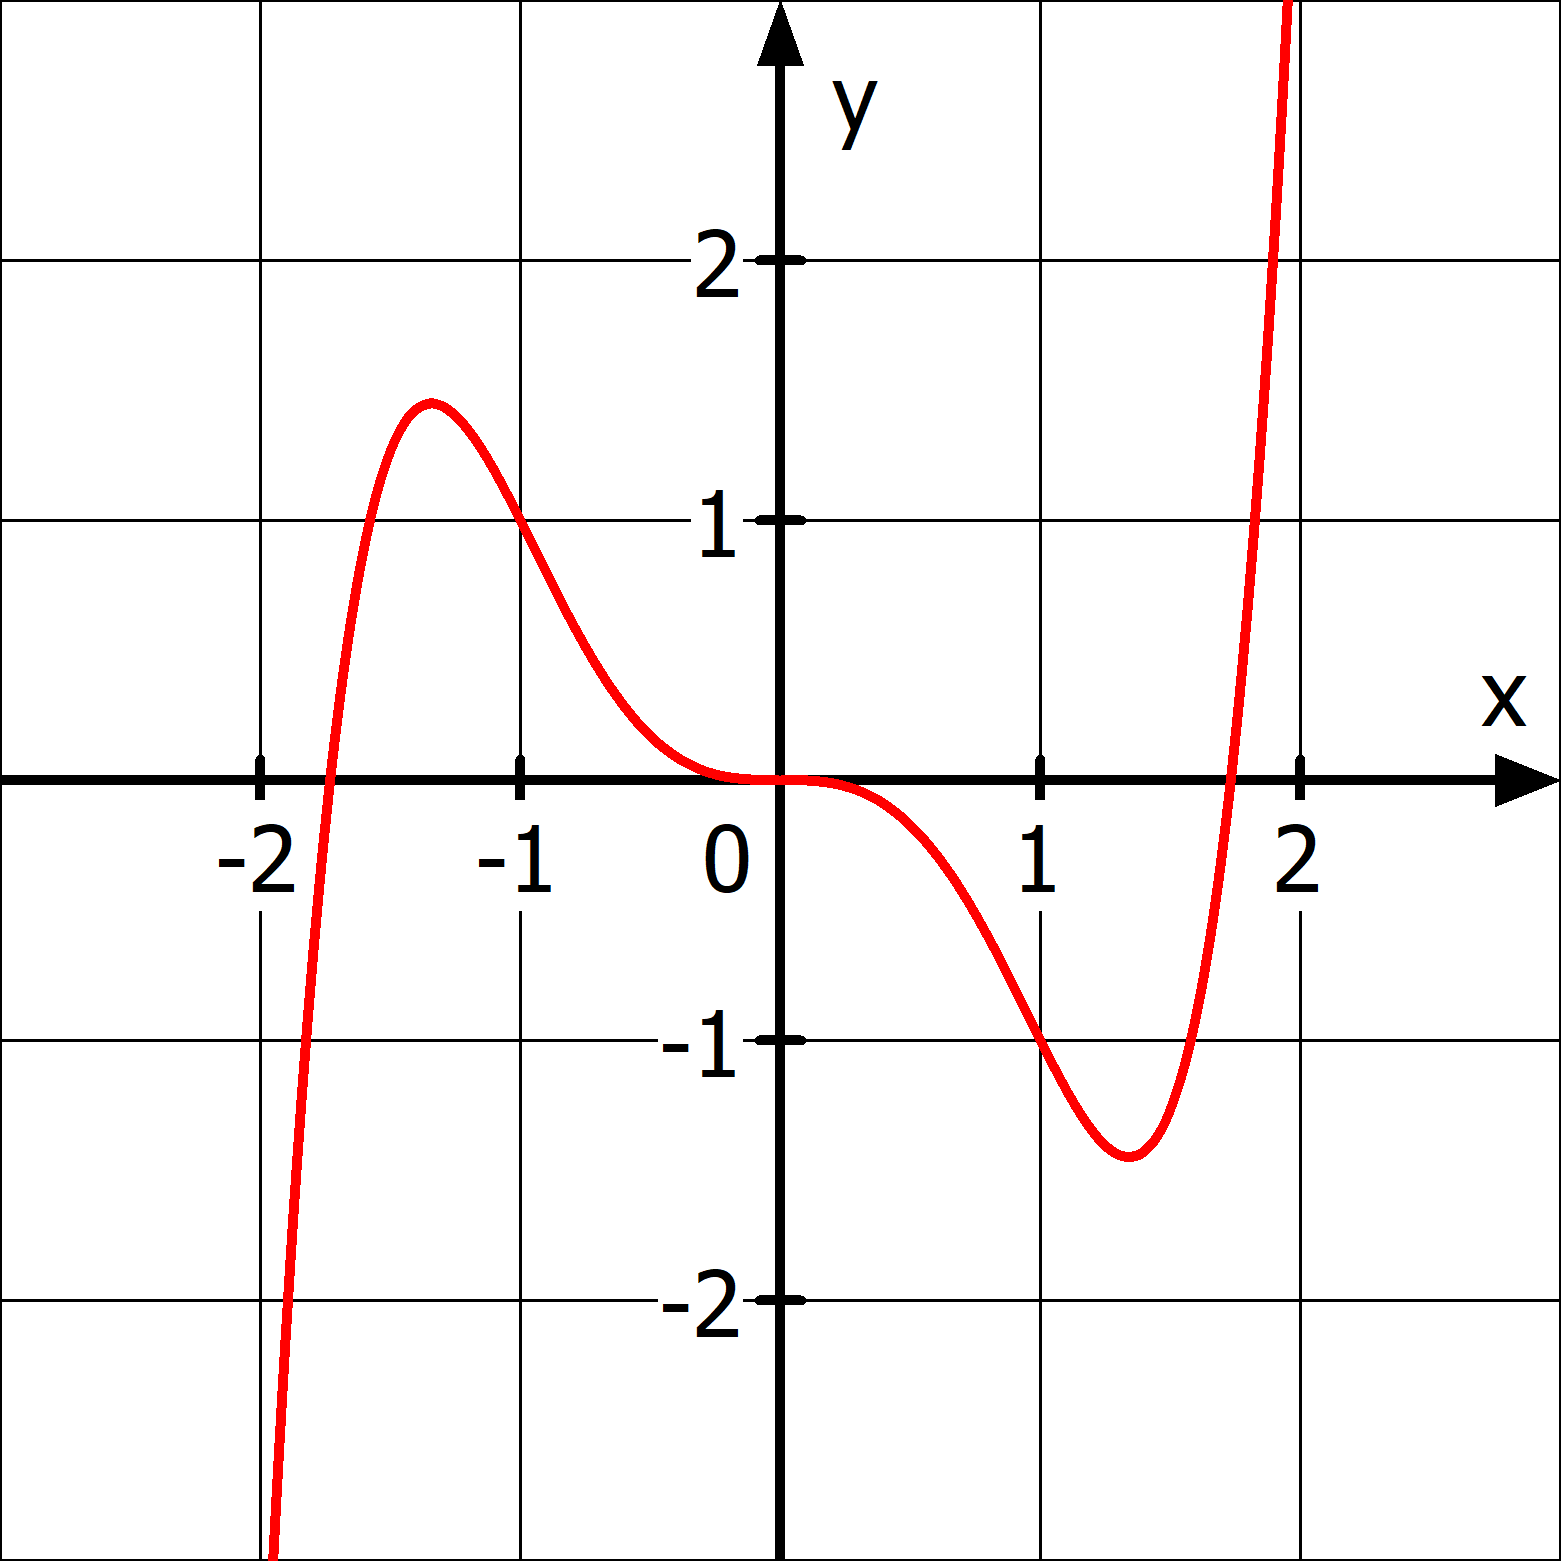
\includegraphics[width=.87\textwidth]{\ganzFkt/pics/sym6.png}

		\(f_8(x)=\frac{1}{2}x^5-\frac{3}{2}x^3\)

		\textcolor{loes}{\(f_8(x)\xrightarrow{\hphantom{\ }x\to-\infty\hphantom{\ }}-\infty\)}

		\textcolor{loes}{\(f_8(x)\xrightarrow{\hphantom{\ }x\to\infty\hphantom{\ }}\infty\)}

		\textcolor{loes}{Verhält sich wie \(\frac{1}{2}x^5\)}
	\end{minipage}}%
	\adjustbox{valign=t}{\begin{minipage}{0.33\textwidth}\centering
		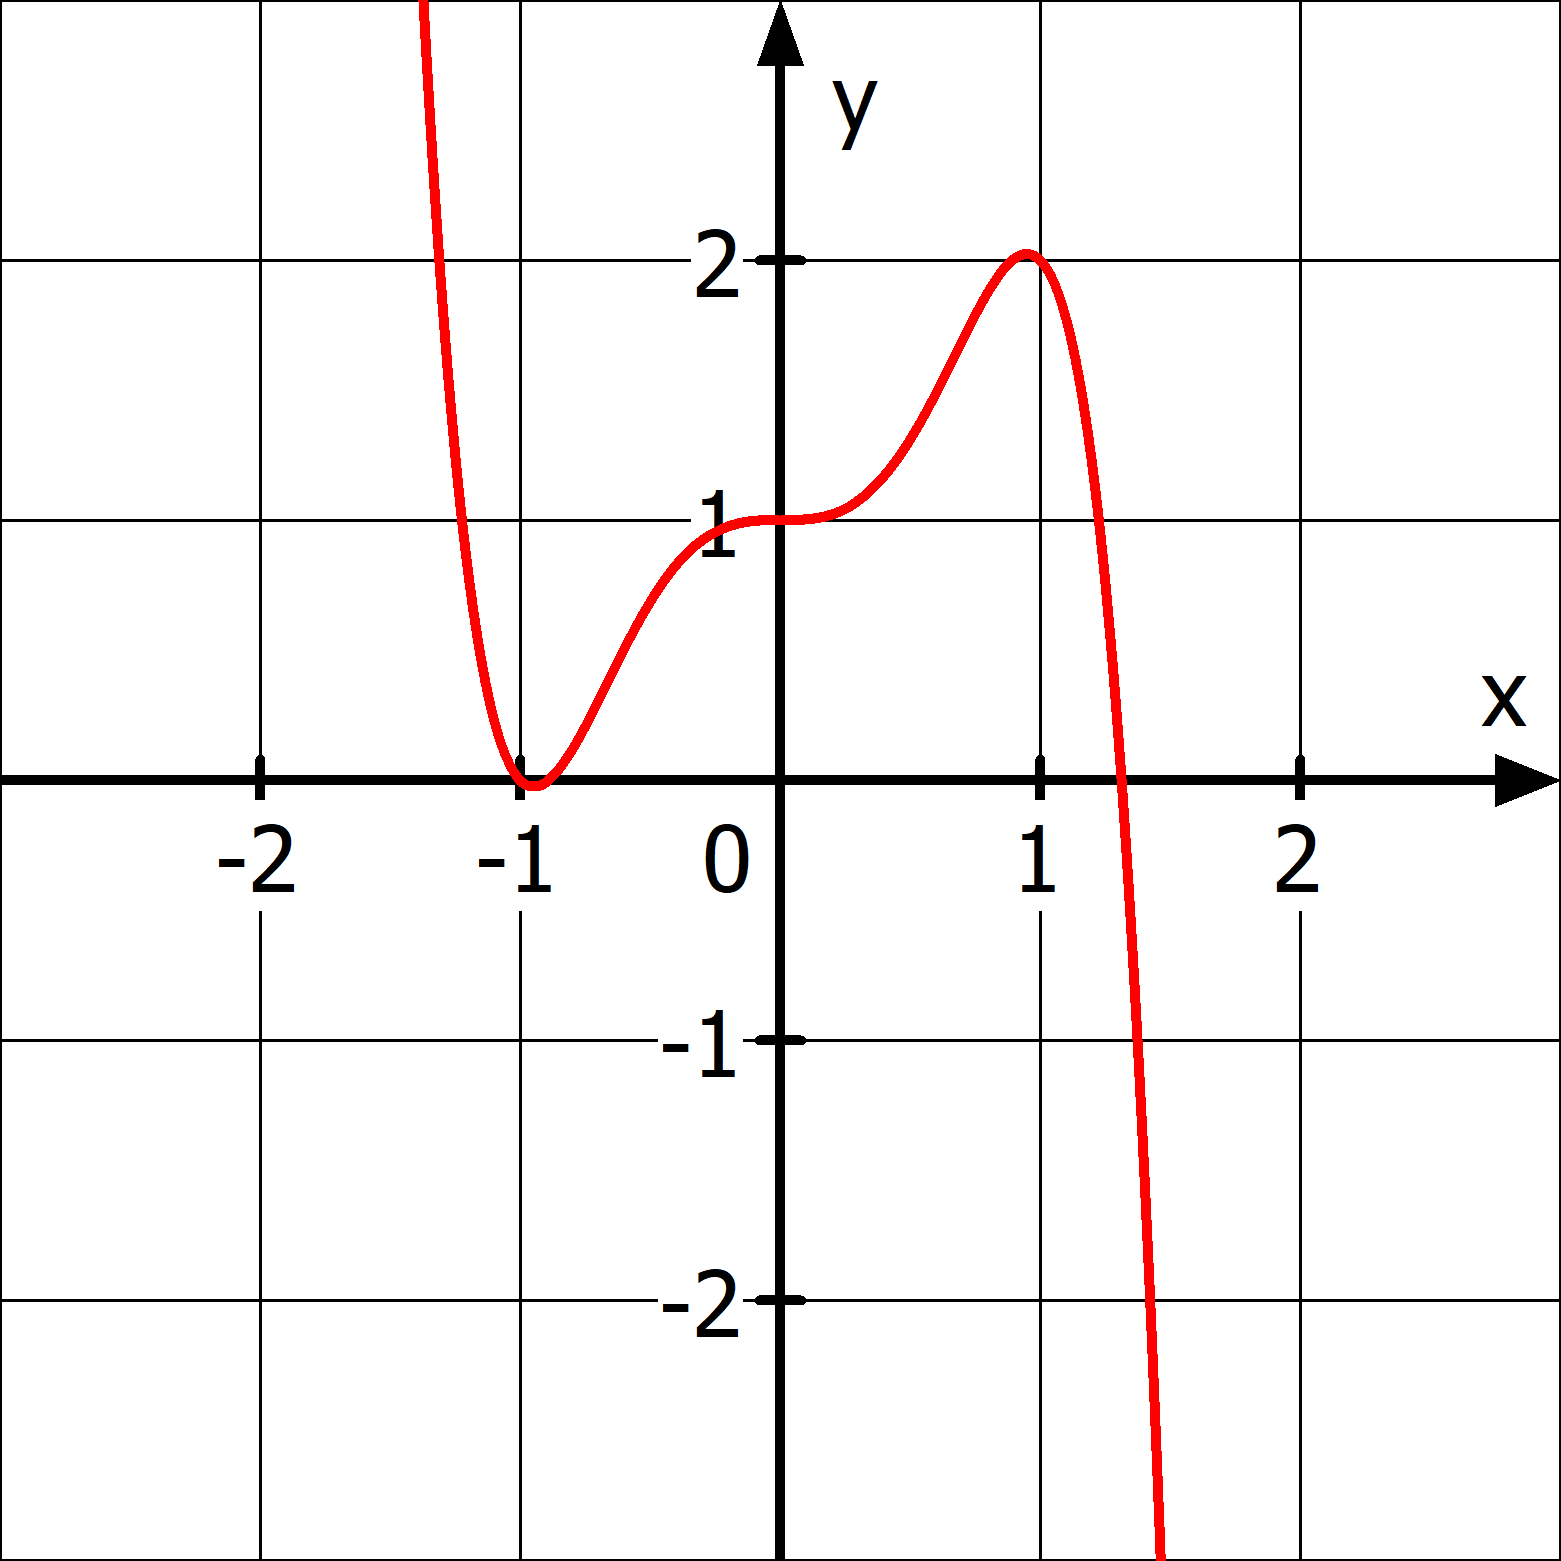
\includegraphics[width=.87\textwidth]{\ganzFkt/pics/sym9.png}

		\(f_9(x)=-2x^5+3x^3+1\)

		\textcolor{loes}{\(f_9(x)\xrightarrow{\hphantom{\ }x\to-\infty\hphantom{\ }}\infty\)}

		\textcolor{loes}{\(f_9(x)\xrightarrow{\hphantom{\ }x\to\infty\hphantom{\ }}-\infty\)}

		\textcolor{loes}{Verhält sich wie \(-2x^5\)}
	\end{minipage}}%
\end{minipage}
%%%%%%%%%%%%%%%%%%%%%%%%%%%%%%%%%%%%%%%%%%%%%%%%%%%%%%%%%%%%%%%%%%%%%%%%%%%%%%%%%%%%%%%%%%%%%%%%%%%%%%%%%%%%%%%%%%%%%
\begin{Exercise}[title={Gib das Verhalten für \(x\to \pm \infty \) an}, label=ganzVerA1]

	\begin{minipage}{\textwidth}
		\begin{minipage}{0.5\textwidth}
			\begin{enumerate}[label=\alph*)]
				\item \(f(x)=3x^3+2x-3\)
				\item \(g(x)=-2,5x^5+5x^3+2,5x^2\)
				\item \(h(x)=2x^6-3x^2-14x+1\)
				\item \(i(x)=-\frac{3}{5}x^5+2x^4+x^2-1\)
			\end{enumerate}
		\end{minipage}%
		\begin{minipage}{0.5\textwidth}
			\begin{enumerate}[label=\alph*)]
				\setcounter{enumi}{4}
				\item \(j(x)=-0,3x^6-x^4+2x^2-5,8\)
				\item \(k(x)=-\frac{7}{5}x^7+\frac{8}{7}x^6-\frac{11}{6}x^2-\frac{12}{5}x\)
				\item \(l(x)=x\left(-x^3+2x^2+5\right)\)
				\item \(m(x)=5x^2\left(x-1\right)^2\)
			\end{enumerate}
		\end{minipage}%
	\end{minipage}
\end{Exercise}
\newpage
%%%%%%%%%%%%%%%%%%%%%%%%%%%%%%%%%%%%%%%%%
\begin{Answer}[ref=ganzVerA1]

	\begin{minipage}{\textwidth}
		\begin{minipage}[t]{0.5\textwidth}
			\begin{enumerate}[label=\alph*)]
				\item Verhält sich wie \(3x^3\)

				\(f(x)\xrightarrow{\hphantom{\ }x\to-\infty\hphantom{\ }}-\infty\)

				\(f(x)\xrightarrow{\hphantom{\ }x\to\infty\hphantom{\ }}\infty\)
				\item Verhält sich wie \(-2,5x^5\)

				\(g(x)\xrightarrow{\hphantom{\ }x\to-\infty\hphantom{\ }}\infty\)

				\(g(x)\xrightarrow{\hphantom{\ }x\to\infty\hphantom{\ }}-\infty\)
				\item Verhält sich wie \(2x^6\)

				\(h(x)\xrightarrow{\hphantom{\ }x\to-\infty\hphantom{\ }}\infty\)

				\(h(x)\xrightarrow{\hphantom{\ }x\to\infty\hphantom{\ }}\infty\)
				\item Verhält sich wie \(-\frac{3}{5}x^5\)

				\(i(x)\xrightarrow{\hphantom{\ }x\to-\infty\hphantom{\ }}\infty\)

				\(i(x)\xrightarrow{\hphantom{\ }x\to\infty\hphantom{\ }}-\infty\)
			\end{enumerate}
		\end{minipage}%
		\begin{minipage}[t]{0.5\textwidth}
			\begin{enumerate}[label=\alph*)]
				\setcounter{enumi}{4}
				\item Verhält sich wie \(-0,3x^6\)

				\(j(x)\xrightarrow{\hphantom{\ }x\to-\infty\hphantom{\ }}-\infty\)

				\(j(x)\xrightarrow{\hphantom{\ }x\to\infty\hphantom{\ }}-\infty\)
				\item Verhält sich wie \(-\frac{7}{5}x^7\)

				\(k(x)\xrightarrow{\hphantom{\ }x\to-\infty\hphantom{\ }}\infty\)

				\(k(x)\xrightarrow{\hphantom{\ }x\to\infty\hphantom{\ }}-\infty\)
				\item \(l(x)=x\left(-x^3+2x^2+5\right)=-x^4+2x^3+5x\)

				Verhält sich wie \(-x^4\)

				\(l(x)\xrightarrow{\hphantom{\ }x\to-\infty\hphantom{\ }}-\infty\)

				\(l(x)\xrightarrow{\hphantom{\ }x\to\infty\hphantom{\ }}-\infty\)
				\item \(m(x)=5x^2\left(x-1\right)^2=5x^4-10x^3+5x^2\)

				Verhält sich wie \(5x^4\)

				\(m(x)\xrightarrow{\hphantom{\ }x\to-\infty\hphantom{\ }}\infty\)

				\(m(x)\xrightarrow{\hphantom{\ }x\to\infty\hphantom{\ }}\infty\)
			\end{enumerate}
		\end{minipage}%
	\end{minipage}
\end{Answer}